\chapter{Problématique et méthodologie de travail}
\markboth{Chapitre 2. Problématique et méthodologie de travail}{} 
\begin{spacing}{1.2}
\minitoc
\thispagestyle{MyStyle}
\end{spacing}
\newpage
\section*{Introduction}
Dans ce chapitre il s'agira pour nous de faire connaitre les fondements de la mise en place de notre plateforme, de faire ressortir la question autour de laquelle gravite notre travail et d'identifier les objectifs que nous nous sommes fixés . \par
\section{Contexte}
La réalisation de notre plateforme numérique s'inscrit dans un contexte où l'accès aux ressources \index{académiques}académiques dans les \index{bibliothèques physiques}bibliothèques physiques pose de nombreux défis. Hormis leur richesse, les bibliothèques traditionnelles souffrent souvent de limitations qui rendent pénible ou entravent l'accès à l'information aux étudiants et chercheurs. Parmi ces limitations, on peut citer la disponibilité restreinte des documents, le nombre limité de copies pour des ouvrages particulièrement demandés, et la difficulté à localiser des mémoires de thèses ou mémoires de master convenable et de qualité.\par
L'accès simultané pour plusieurs personnes à une même ressource est un problème récurrent dans les bibliothèques physiques. Lorsqu'un ouvrage ou un mémoire est particulièrement sollicité, les étudiants peuvent se retrouver en liste d'attente ou se heurter à l'indisponibilité des documents. Cette situation freine le progrès des recherches et la préparation des travaux académiques.\par
De plus, le manque ou la difficulté à trouver des thèses et mémoires dignes d'intérêt est un autre obstacle majeur. Les étudiants doivent souvent consacrer un temps considérable à fouiller parmi des centaines de documents pour identifier ceux qui correspondent le mieux à leurs besoins spécifiques. Ce processus peut être laborieux et décourageant, surtout lorsque les ressources disponibles sont dispersées et mal cataloguées.
\par
\section{Problématique}

Trouver un mémoire de thèse ou un mémoire de master convenable actuellement à l'UNZ nécessite non seulement une présence physique à la bibliothèque, mais également la disponibilité du document qui nous intéresse et aussi qu'il soit en bon état. Au vu de la place importante qu'occupe la recherche, il serai judicieux de rendre plus aisé l'accès et l'exploitation des mémoires de thèse et master. Le numérique vient alors résoudre le problème avec la possibilité de stocker ces ressources au format numérique et de les rendre facilement accessible offrant ainsi plusieurs avantages. 
Grâce à la mise en ligne des ressources, non seulement les mémoires seront sur de demeurer en bon état mais ils seront accessible par un grand nombre d'utilisateur sans se soucier de leur disponibilité. 
\par
\section{Objectifs}
\textbf{Objectif principal :} Notre objectif principal est de rendre disponible en ligne le format numérique des mémoires de thèse et mémoires de master.

\textbf{Objectif secondaire 1 :} Comme objectif secondaire numéro un il s'agira de mettre en place un système sécurisé de stockage des mémoires de thèses et mémoires de master au format PDF en ligne.

\textbf{Objectif secondaire 2 :} Notre objectif secondaire numéro deux sera de concevoir une solution numérique permettant de rechercher, lire et télécharger des documents au format PDF en ligne.

\textbf{Objectif secondaire 3 :} Notre objectif secondaire numéro trois sera de créer un moyen permettant aux membres de la communauté universitaire de pouvoir exposer leur incompréhension de certaines parties des mémoires de thèses ou mémoire de master afin de bénéficier des explications des auteurs.
 \par
 
De nos objectifs, nous avons les avantages suivants :  
 
\textbf{Avantage du stockage en ligne des mémoires de thèses et mémoires de master en ligne}
La conservation des documents au format numérique représente un tournant majeur dans la gestion et la préservation du patrimoine académique et offre plusieurs avantages. Opter pour cette approche permettra de :\par

	- Préserver l'intégrité des documents dans des conditions optimales. Contrairement aux supports physiques qui sont sujets à la détérioration, à la perte ou au vol.\par
	- Stocker et sauvegarder les fichiers numériques de manière sécurisée, réduisant ainsi les risques de perte de données précieuses. De plus, grâce aux technologies de sauvegarde et de stockage en ligne, il est possible de créer des copies de sauvegarde afin de garantir la pérennité des documents, même en cas de sinistre.\par

	- Faciliter l’accès pour les utilisateurs. Avec une simple connexion à internet, les acteurs la communauté universitaire peuvent consulter et télécharger les documents.\par
	- Rendre disponible de façon permanent(24/7) les documents et Réduire les coûts d'impression et de stockage. Les documents numériques éliminent les coûts liés à l'impression, au papier et au stockage physique.
  
Notre premier objectif secondaire est donc d’assurer la mise en ligne des documents (résultats des travaux de recherches) ce qui va engendrer une facilité d'accès qui transcende les frontières physiques des bibliothèques traditionnelles, permettant ainsi aux utilisateurs d'explorer un vaste ensemble de ressources documentaires sans contraintes.

\textbf{Avantage d'une solution numérique permettant de rechercher, lire et télécharger des documents au format PDF en ligne}
 Mettre en place un moyen de rechercher, lire et télécharger des documents au format PDF en ligne présente plusieurs avantages tels que: \par
 -Accélérer la recherche. Les fonctions de recherche avancée permettent de trouver rapidement des documents à l'aide de mots-clés des thème ou des identifiants.\par 
 
 - Simplifier la découverte d'une thèse ou un mémoire qui répond au besoin.\par
 
 - Avoir facilement une idée des thèmes déjà traités.
 
 - Faire de recherche avancées, facilitant la découverte et l'exploration des documents. \par
 
	Notre objectif secondaire numéro deux est donc de mettre en place un système numériques permettant aux utilisateurs de trouver rapidement des documents pertinents en utilisant des mots-clés de recherche. Cette fonctionnalité de recherche améliorée contribue à optimiser l'efficacité de la recherche académique, en permettant aux utilisateurs de découvrir plus facilement des travaux pertinents dans leur domaine d'intérêt et de gagner considérablement en temps.\par


\textbf{Avantage d'un espace pour les échange entre les acteurs de la communauté universitaire.}
Notre objectif secondaire numéro trois qui est de créer un espace d'échange dynamique et enrichissant entre les auteurs de la communauté universitaire est aussi essentiel car cela facilitera la progression des recherche.
Grâce à cet espace, il sera possible de: \par 

	- Avoir un espace où chacun pourra apprécier les travaux ou exposer ses différentes préoccupations afin que les auteurs puissent répondre aux questions, clarifier les points complexes.\par
	- Echanger des idées novatrices entre les acteurs de la communauté universitaire.\par
	Bénéficier directement des connaissances et des perspectives des auteurs, enrichissant ainsi leur compréhension et leur engagement.\par

En mettant en avant cet objectif, nous aspirons à créer une plateforme qui transcende les barrières traditionnelles de la recherche académique, favorisant une culture de collaboration, de transparence et d'ouverture. Par cette approche, nous visons à renforcer les liens entre les membres de la communauté universitaire, à promouvoir une compréhension plus approfondie des travaux de recherche et à catalyser l'innovation et le progrès dans notre communauté universitaire.\par

En somme, les objectifs de notre plateforme visent à répondre à un besoin essentiel dans le domaine de la recherche académique : celui de créer un espace dynamique où la numérisation des travaux de recherche et la collaboration entre les auteurs et la communauté universitaire peuvent prospérer. En favorisant la diffusion transparente, et sécurisé des connaissances et en encourageant les échanges constructifs et la coopération entre les acteurs de la communauté universitaire, nous aspirons à travers notre plateforme, à stimuler l'innovation, à renforcer les liens au sein de la communauté universitaire et à contribuer à l'avancement global de la recherche. 

\section{Méthodologie de travail}
Ici, nous décrirons notre méthodologie de travail, détaillant les principes directeurs, les processus et les pratiques adopté pour mener à bien la création de notre plateforme numérique. En présentant notre méthodologie nous visons à offrir un aperçu complet de notre processus de développement, mettant en lumière les stratégies que nous avons adoptées pour assurer le succès de notre projet.

\subsection{Présentation de la méthodologie agile Scrum}
La méthodologie Agile Scrum est une approche de gestion de projet qui vise à favoriser la flexibilité, la réactivité et la collaboration dans le développement de produits logiciels et de solutions complexes. Contrairement aux autres méthodologies , Scrum privilégie une approche itérative et incrémentale, où le travail est organisé en cycles courts appelés "sprints"\cite{permana2015scrum}.
	Au cœur de cette méthodologie se trouvent trois principaux acteurs dont nous endosserons le rôle : le Product Owner, l'Équipe de développement et le Scrum Master. Le Product Owner est chargé de définir les objectifs du projet et de prioriser les fonctionnalités à développer, en se basant sur les besoins du client et les retours utilisateurs. L'Équipe de développement est responsable de la réalisation des tâches et de la livraison des fonctionnalités lors de chaque sprint. Le Scrum Master, quant à lui, est garant du respect des principes Scrum, il facilite les interactions au sein de l'équipe et veille à ce que les processus Scrum soient bien compris et suivis.
La méthodologie Scrum repose également sur un ensemble d'artefacts et d'événements clés. Les principaux artefacts incluent le Product Backlog, qui recense toutes les fonctionnalités à développer, et le Sprint Backlog, qui contient les tâches à réaliser lors de chaque sprint. Les événements Scrum comprennent la Planification du Sprint, qui définit les objectifs du sprint, le Daily Scrum, une réunion quotidienne pour synchroniser le travail de l'équipe, la Revue de Sprint, où les fonctionnalités développées sont présentées au Product Owner, et la Rétrospective de Sprint, qui permet à l'équipe de réfléchir et de s'améliorer continuellement.
En résumé, la méthodologie Agile Scrum offre une approche structurée et adaptable pour gérer efficacement les projets complexes. En favorisant la maneabilité, et la livraison continue de valeur, Scrum permet au développeur d'organiser et de générer plus facilement les tâches à travers des solutions adaptatives pour des problèmes complexes \cite{schwaber2011scrum}.
	
	
	
	\begin{figure}[H]%
    \center%
    \setlength{\fboxsep}{5pt}%
    \setlength{\fboxrule}{0.5pt}%
    \fbox{
    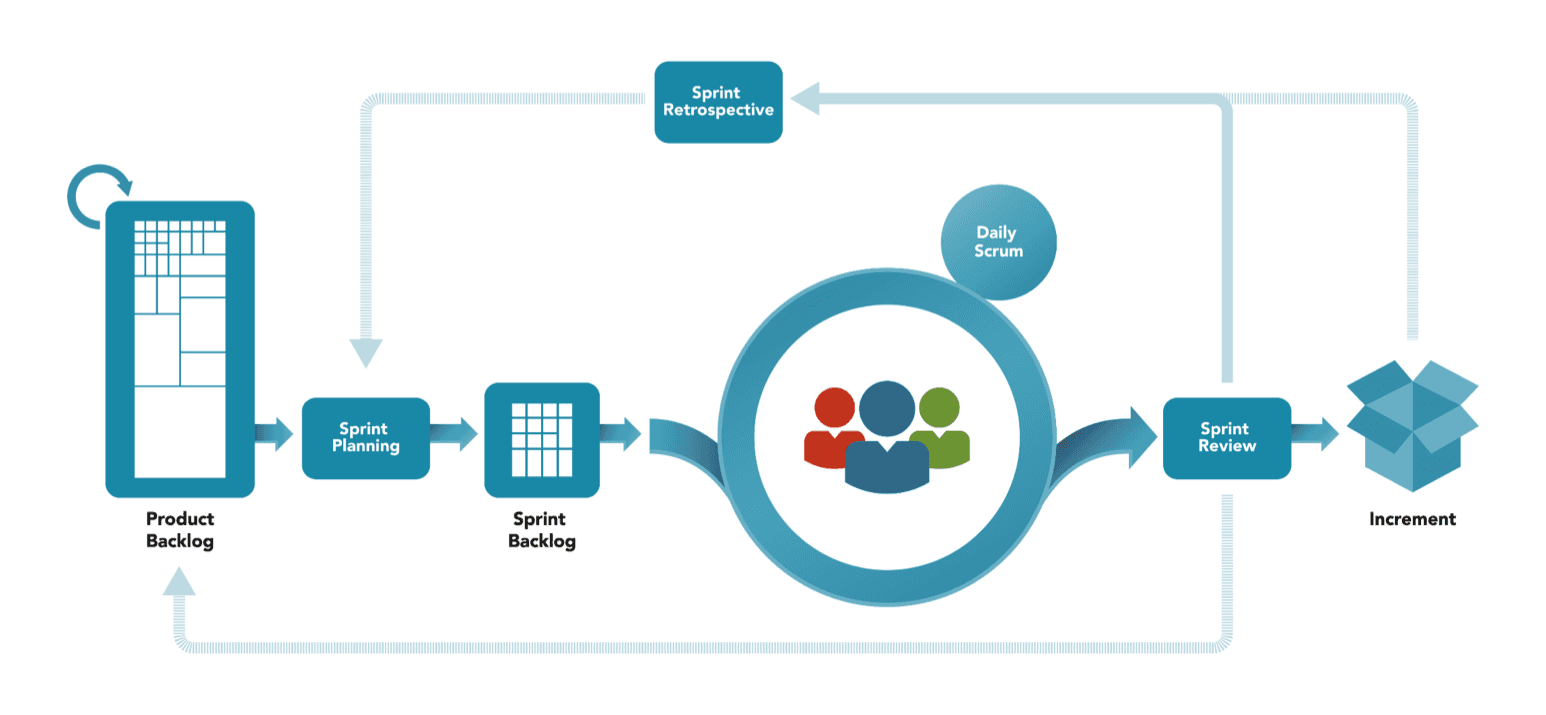
\includegraphics[width=14cm,height=8.5cm]{images/scrum.png}%
    }
    \caption{Fonctionnement de la méthodologie agile scrum}%
\end{figure}

\textbf{Description du fonctionnement :}

\textbf{- Product Backlog :} Une liste dans laquelle on recense tout ce qui pourrait être nécessaire dans le produit. Il est constamment mis à jour et affiné.

\textbf{- Sprint Planning :} Une réunion est faite au début de chaque sprint où l'on planifie le travail à accomplir durant le sprint. Les objectifs du sprint et le Sprint Backlog sont définis.\par

 \textbf{- Sprint Backlog :} Ensemble des éléments du Product Backlog sélectionnés pour le sprint, ainsi qu'un plan pour les délivrer. Il est créé lors de la Sprint Planning Meeting. 
 \par

\textbf{- Daily Scrum :} Réunion quotidienne de 15 minutes pour synchroniser les activités et planifier les prochaines 24 heures. On répond à trois questions : Qu'ai-je fait hier ? Que vais-je faire aujourd'hui ? Quels sont les obstacles ?
 \par 
 
\textbf{- Sprint Review :} Réunion à la fin du sprint où l'incrément est présenté pour recueillir des commentaires. Le Product Backlog peut être ajusté en fonction des retours.
 \par  
 
 \textbf{- Sprint Retrospective :} Réunion après la Sprint Review et avant le début du prochain sprint où l'on réfléchit sur le sprint écoulé et identifie des améliorations pour les prochains sprints.
 \par 
 
 \textbf{- Increment  :}  La somme de tous les éléments du Product Backlog complétés durant un sprint et les incréments des sprints précédents. À la fin de chaque sprint, l'incrément doit être "Done" (fini) et potentiellement livrable.
 \par  
 

\section*{Conclusion}

En conclusion, la mise en place de notre plateforme numérique des mémoires de thèses et mémoires de master répond à une nécessité pressante de faciliter l'accès aux ressources académiques en les mettant en ligne dans un contexte où les bibliothèques physiques présentent de nombreuses limitations. En transformant ces documents en ressources numériques, nous offrons une solution efficace pour surmonter les obstacles liés à la disponibilité restreinte et à l'accès limité aux ouvrages de qualité.\par

Notre démarche s'articule autour de trois objectifs secondaire aboutissant à un objectif principal. \par 

 Le premier secondaire est de mettre en place un moyen fiable et sécurisé de stockage en ligne au format PDF des mémoires de thèses et mémoires de master. Ce qui va garantir la conservation à long terme des travaux de recherche tout en facilitant leur accès à un public plus large grâce aux avantages du numérique.\par 

Le deuxième objectif secondaire est de concevoir un système de recherche pour un filtrage efficace permettant de réduire rapidement les résultats de recherche à ceux qui sont les plus pertinents, économisant ainsi du temps.
 
 Ce passage au format numérique permet non seulement de préserver les documents dans des conditions optimales, mais aussi de les rendre accessibles de partout et à tout moment, tout en intégrant des fonctionnalités de recherche avancées pour optimiser l'efficacité des recherches académiques.\par

Le troisième objectif secondaire vise à créer un cadre d'échange enrichissant entre les acteurs de la communauté universitaire. En créant un espace interactif sur notre plateforme, nous encourageons un dialogue ouvert et constructif, permettant aux utilisateurs de poser des questions, d'obtenir des clarifications et d'échanger des idées novatrices.\par

Ainsi, notre plateforme aspire à transcender les barrières traditionnelles de la recherche académique, en offrant une solution numérique intégrée qui répond aux besoins de conservation, d'accès, de filtrage et de collaboration.
\par

Pour pouvoir atteindre nos objectifs, nous avons adopter la méthodologie agile scrum. Cette méthodologie nous a permis de travailler de manière flexible fluide.